\section*{Desenvolvimento}

O desenvolvimento do projeto foi dividido em três etapas principais: pré-processamento dos dados, definição das métricas de avaliação e, por fim, o treinamento e otimização dos modelos.

\subsection*{1. Pré-processamento e Análise}
A qualidade dos dados de entrada é fundamental para o desempenho do modelo, sendo assim, fizemos uma análise das colunas para extrair o máximo de informação possivel.

\paragraph{Tratamento de Dados Ausentes:} Uma análise inicial revelou que o atributo \texttt{other\_support\_plans} continha 649 valores ausentes em 800 amostras (mais de 81\%).
Devido ao grande numero de valores faltantes, usar eles como input seria pouco confiável.
Portanto, esta coluna foi removida do conjunto de dados.

\paragraph{Análise da Variável target:} A variável target \texttt{support\_outcome} mostrou-se desbalanceada, com 70\% das amostras classificadas como "good" e 30\% como "bad".

\paragraph{Codificação de Atributos Categóricos:} Os atributos categóricos foram tratados de acordo 
com sua natureza (nominal ou ordinal) usando um \texttt{ColumnTransformer} do Scikit-learn.
\begin{itemize}
    \item \textbf{Atributos Ordinais:} Atributos com uma ordem intrínseca (ex: \texttt{garden\_points\_status}, \texttt{personal\_reserve\_status}, \texttt{role\_skill\_tier}) foram codificados usando \texttt{OrdinalEncoder} para preservar sua relação de classificação.
    \item \textbf{Atributos Nominais:} Atributos sem ordem (ex: \texttt{project\_focus\_code}, \texttt{housing\_situation}) foram codificados usando \texttt{OneHotEncoder} para criar variáveis "dummy".
\end{itemize}
Os atributos numéricos foram mantidos em sua escala original (\texttt{passthrough}), exceto para o modelo SVM, pois os modelos baseados em árvore não são sensíveis à escala dos atributos. O \texttt{id} foi removido. O dataset processado final contém 48 atributos.
\vspace{5mm}
\subsection*{2. Métricas de Avaliação}
No fito de comparar os modelos, utilizamos duas métricas padrão para classificação.

\paragraph{Acurácia (Accuracy):} Mede a proporção de previsões corretas sobre o total. É definida como:
$$ \text{Acurácia} = \frac{VP + VN}{VP + VN + FP + FN} $$
Onde $VP$ (Verdadeiro Positivo) e $VN$ (Verdadeiro Negativo) são as classificações corretas, e $FP$ (Falso Positivo) e $FN$ (Falso Negativo) são os erros.

\paragraph{Área sob a Curva ROC (AUC-ROC):} A AUC-ROC é uma medida robusta utilizada em problemas de classificação, gerada ao variar o threshold de um classificador e calculando a área da curva final. A curva ROC plota a Taxa de Verdadeiros Positivos (TPR) contra a Taxa de Falsos Positivos (FPR) em vários limiares de decisão, sendo mais próximo de 1 melhor.
$$ \text{TPR (Sensibilidade)} = \frac{VP}{VP + FN} $$
$$ \text{FPR} = \frac{FP}{FP + VN} $$
Iremos sempre comparar a AUC em relação ao modelo aleatório, considerando-se que ele terá AUC de 0.5. Se for maior que 0.5, representa que o modelo tem alguma capacidade preditiva melhor que o modelo randômico.
\vspace{5mm}
\subsection*{3. Modelos Baseados em Árvore}
Estes modelos funcionam dividindo sequencialmente os dados com base nos limiares dos atributos. A "qualidade" de uma divisão é medida por critérios de impureza (Gini ou Entropia).

\subsubsection*{Modelo 1: Árvore de Decisão}
Uma única árvore de decisão foi treinada e otimizada via \texttt{GridSearchCV}.
O modelo atingiu uma \textbf{Acurácia Cross-Validation de 0.7031}  e uma \textbf{AUC de 0.6585}.
Este desempenho, o mais baixo entre os modelos testados, é esperado, pois árvores únicas tendem a ter alta variância e sobreajustar (overfit) aos dados de treino. Sendo assim, a idéia do trabalho foi testar algoritmos como o Random Forest, que irão reduzir essa variância das árvores de decisão.
\vspace{5mm}
\subsubsection*{Modelo 2: Floresta Aleatória (Random Forest)}
Este modelo de ensemble (ensemble é a composição de N modelos para criar um preditor ou regressor final) reduz a variância ao construir múltiplas árvores de decisão em subconjuntos aleatórios dos dados e atributos.
Após a otimização com \texttt{GridSearchCV}, o modelo alcançou a 3ª maior acurácia: uma \textbf{Acurácia Cross-Validation de 0.7437}  e a melhor \textbf{AUC de 0.7842}. 
Os melhores hiperparâmetros encontrados foram: \texttt{'max\_depth': 20}, \texttt{'max\_features': sqrt}, \texttt{'min\_samples\_leaf': 3}, \texttt{'min\_samples\_split': 2}, \texttt{'n\_estimators': 200}.
\vspace{5mm}
\subsubsection*{Modelo 3: Aumento de Gradiente (Gradient Boosting)}
Este modelo também de ensemble constrói árvores sequencialmente, onde cada nova árvore corrige os erros residuais da árvore anterior. Esse modelo tem como objetivo combinar weak learners para reduzir o viés de um modelo, diferentemente do Random Forest que tem como objetivo redzuria  variância das árvores.
A otimização com \texttt{GridSearchCV} resultou em uma \textbf{Acurácia Cross-Validation de 0.7578}  e uma \textbf{AUC de 0.7440}.
Os melhores hiperparâmetros encontrados foram: \texttt{'learning\_rate': 0.05}, \texttt{'max\_depth': 20}, \texttt{'min\_samples\_leaf': 10}, \texttt{'min\_samples\_split': 5}, \texttt{'n\_estimators': 200}.
\vspace{5mm}
\subsection*{4. Modelo Probabilístico: Naive Bayes}
O classificador Naive Bayes é um modelo probabilístico baseado no Teorema de Bayes, que assume que os atributos são independentes, resultando em um reduzido custo computacional. Esse modelo, por assumir dados independentes e geralmente gerados por distribuições normais, é considerado ter um alto viés.
Utilizamos o \texttt{GaussianNB}, que assume que os atributos contínuos seguem uma distribuição normal.
Este modelo foi notavelmente rápido. Ele alcançou \textbf{Acurácia Cross-Validation de 0.7312},e uma \textbf{AUC de 0.7539}. O melhor hiperparâmetro encontrado foi: \textbf{Var smoothing de 1e-08}.
\vspace{5mm}
\subsection*{5. Máquina de Vetor de suporte}
O classificador SVM (Support Vector Machine) funciona encontrando o hiperplano que melhor separa as classes no espaço de atributos, maximizando a margem entre o hiperplano e os pontos de dados mais próximos de cada classe, conhecidos como vetores de suporte. 
Os melhores hiperparâmetros encontrados foram: \textbf{C = 100} e \textbf{gamma = 0.001}.
\vspace{5mm}
\subsection*{6. Classificador de votação}
O Classificador de Votação (Voting Classifier) é um modelo de ensemble learning que combina as previsões de vários modelos base para produzir uma previsão final. Seu objetivo é aumentar a robustez e a precisão geral do sistema, aproveitando a força individual de diferentes algoritmos e mitigando suas fraquezas. 
Nesta implementação, o classificador de votação opera no modo 'soft voting' (votação ponderada). Foram escolhidos os 3 modelos com os maiores AUC para funcionarem como estimadores-base para este modelo: Random forest (peso = 3), Gradient Boosting (peso = 2) e Gaussian Naive Bayes (peso = 1)

Cada estimador-base gera a probabilidade de uma amostra ser classificada em cada uma das classes. A média ponderada pelos pesos acima é calculada para cada classe. O resultado é classe que tem a maior probabilidade.
\vspace{5mm}
\subsection*{7. Análise Visual dos Resultados}
As matrizes de confusão (Figuras 1 e 2) fornecem uma visão detalhada dos erros de cada modelo no conjunto de validação.
A Figura 1(a) (Árvore de Decisão) mostra uma tendência em classificar "good" como "bad" (30 Falsos Negativos) com mais frequência do que o inverso (26 Falsos Positivos) , enquanto os modelos de ensemble (Figuras 1(b) e 2(a)) são mais balanceados.

\begin{figure}[H]
    \centering
    \subfloat[Decision Tree \\ (CV Acc: 0.7031)]{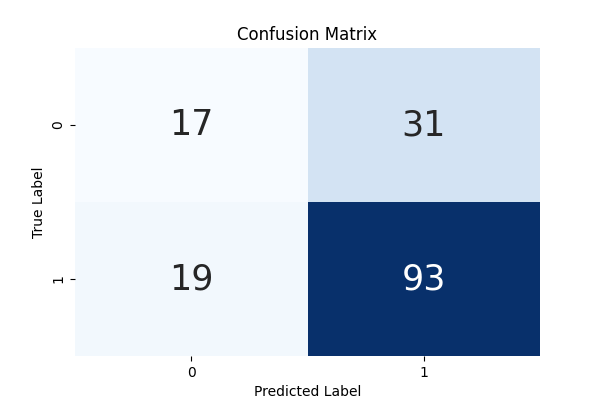
\includegraphics[width=0.3\linewidth]{results/Decision Tree_confusion_matrix.png}\label{fig:conf_dt}}
    \subfloat[Random Forest \\ (CV Acc: 0.7437)]{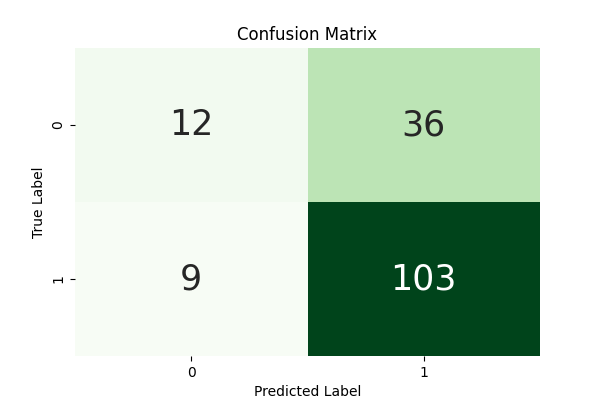
\includegraphics[width=0.3\linewidth]{results/Random Forest_confusion_matrix.png}\label{fig:conf_rf}}
    \subfloat[Gradient Boosting \\ (CV Acc: 0.7578)]{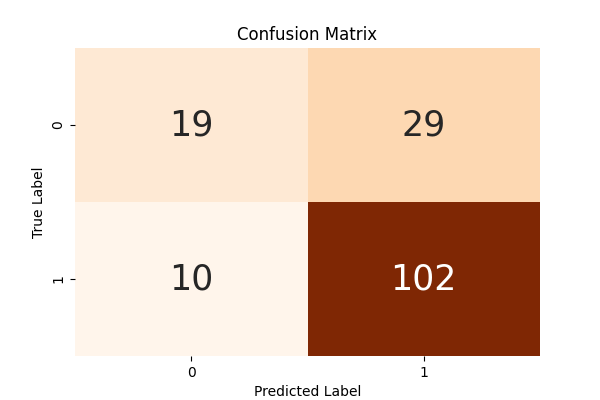
\includegraphics[width=0.3\linewidth]{results/Gradient Boosting_confusion_matrix.png}\label{fig:conf_gb}}
\end{figure}
\begin{figure}[H]
    \centering
    \subfloat[Gaussian Naive Bayes \\ (CV Acc: 0.7312)]{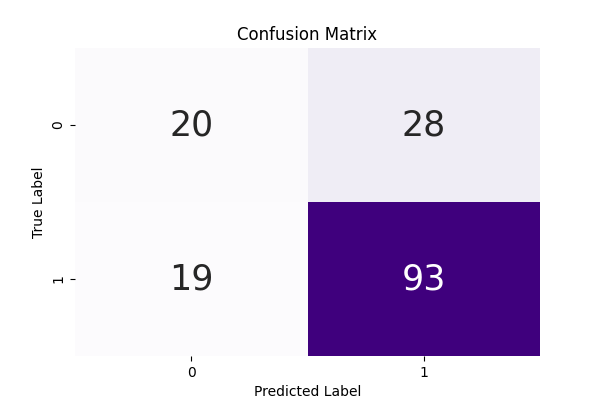
\includegraphics[width=0.3\linewidth]{results/Gaussian Naive Bayes_confusion_matrix.png}\label{fig:conf_dt}}
    \subfloat[Support Vector Machine \\ (CV Acc: 0.7281)]{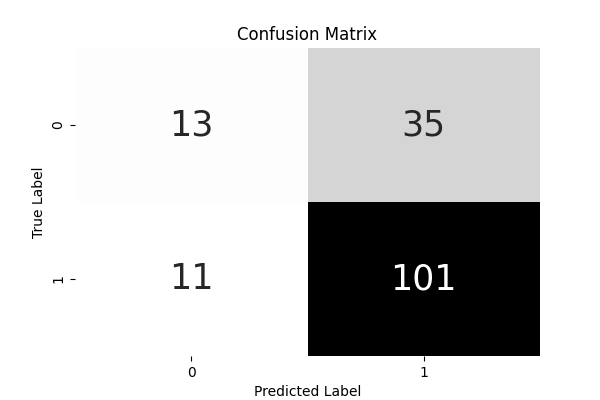
\includegraphics[width=0.3\linewidth]{results/Support Vector Machine_confusion_matrix.png}\label{fig:conf_rf}}
    \subfloat[Voting Classifier \\ (CV Acc: 0.7593)]{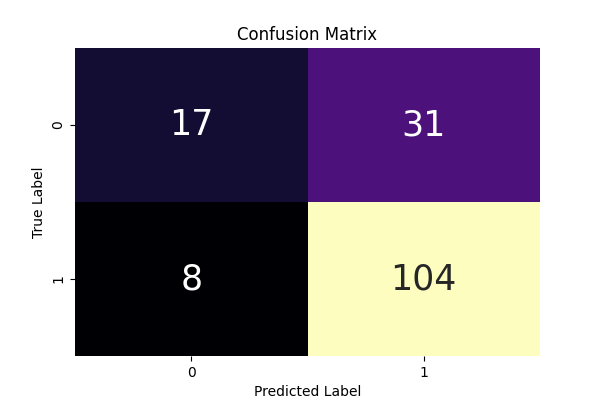
\includegraphics[width=0.3\linewidth]{results/Voting Classifier_confusion_matrix.png}\label{fig:conf_gb}}
\end{figure}
